\chapter{Media Bias}
\label{cha:2}

\section{Definition} \label{media-bias-definition}

Allsides \cite{allsides-2022-bias-definition} defines media bias as "The tendency of news media to report in a way that reinforces a viewpoint, worldview, preference, political ideology, corporate or financial interests, moral framework, or policy inclination, instead of reporting in an objective way (simply describing the facts)". This phenomenon has existed and been researched since the 1950s \cite{white-1950-case-study-selection-news}, highlighting its enduring presence and impact on public perception. Media bias can manifest in various forms, including the selection of stories, framing of issues, and choice of language.

While biases may not always be intentional, they might cause significant consequences, possibly leading to inequalities and injustices. Some news outlets tend to use catchy headlines which trick readers into clicking, known as "clickbait", which are often ambiguous or misleading. Biased information can and has been used as a way to shape and influence public opinion \cite{aires-2020-information}. A survey of journalists from the United States, Great Britain, Germany, Italy, and Sweden found evidence that journalists' personal beliefs substantially influence their news decisions, expressed within the stories they choose and the statements they write \cite{patterson-donsbach-1996-news-decisions}.

Media bias can manifest within different levels, categorised into 4 major types \cite{spinde-2024-taxonomy}, as shown in Figure \ref{fig:bias-types-taxonomy}.

\begin{comment}
Explain types of bias one by one?
\end{comment}

\begin{figure}[htbp]
    \centering
    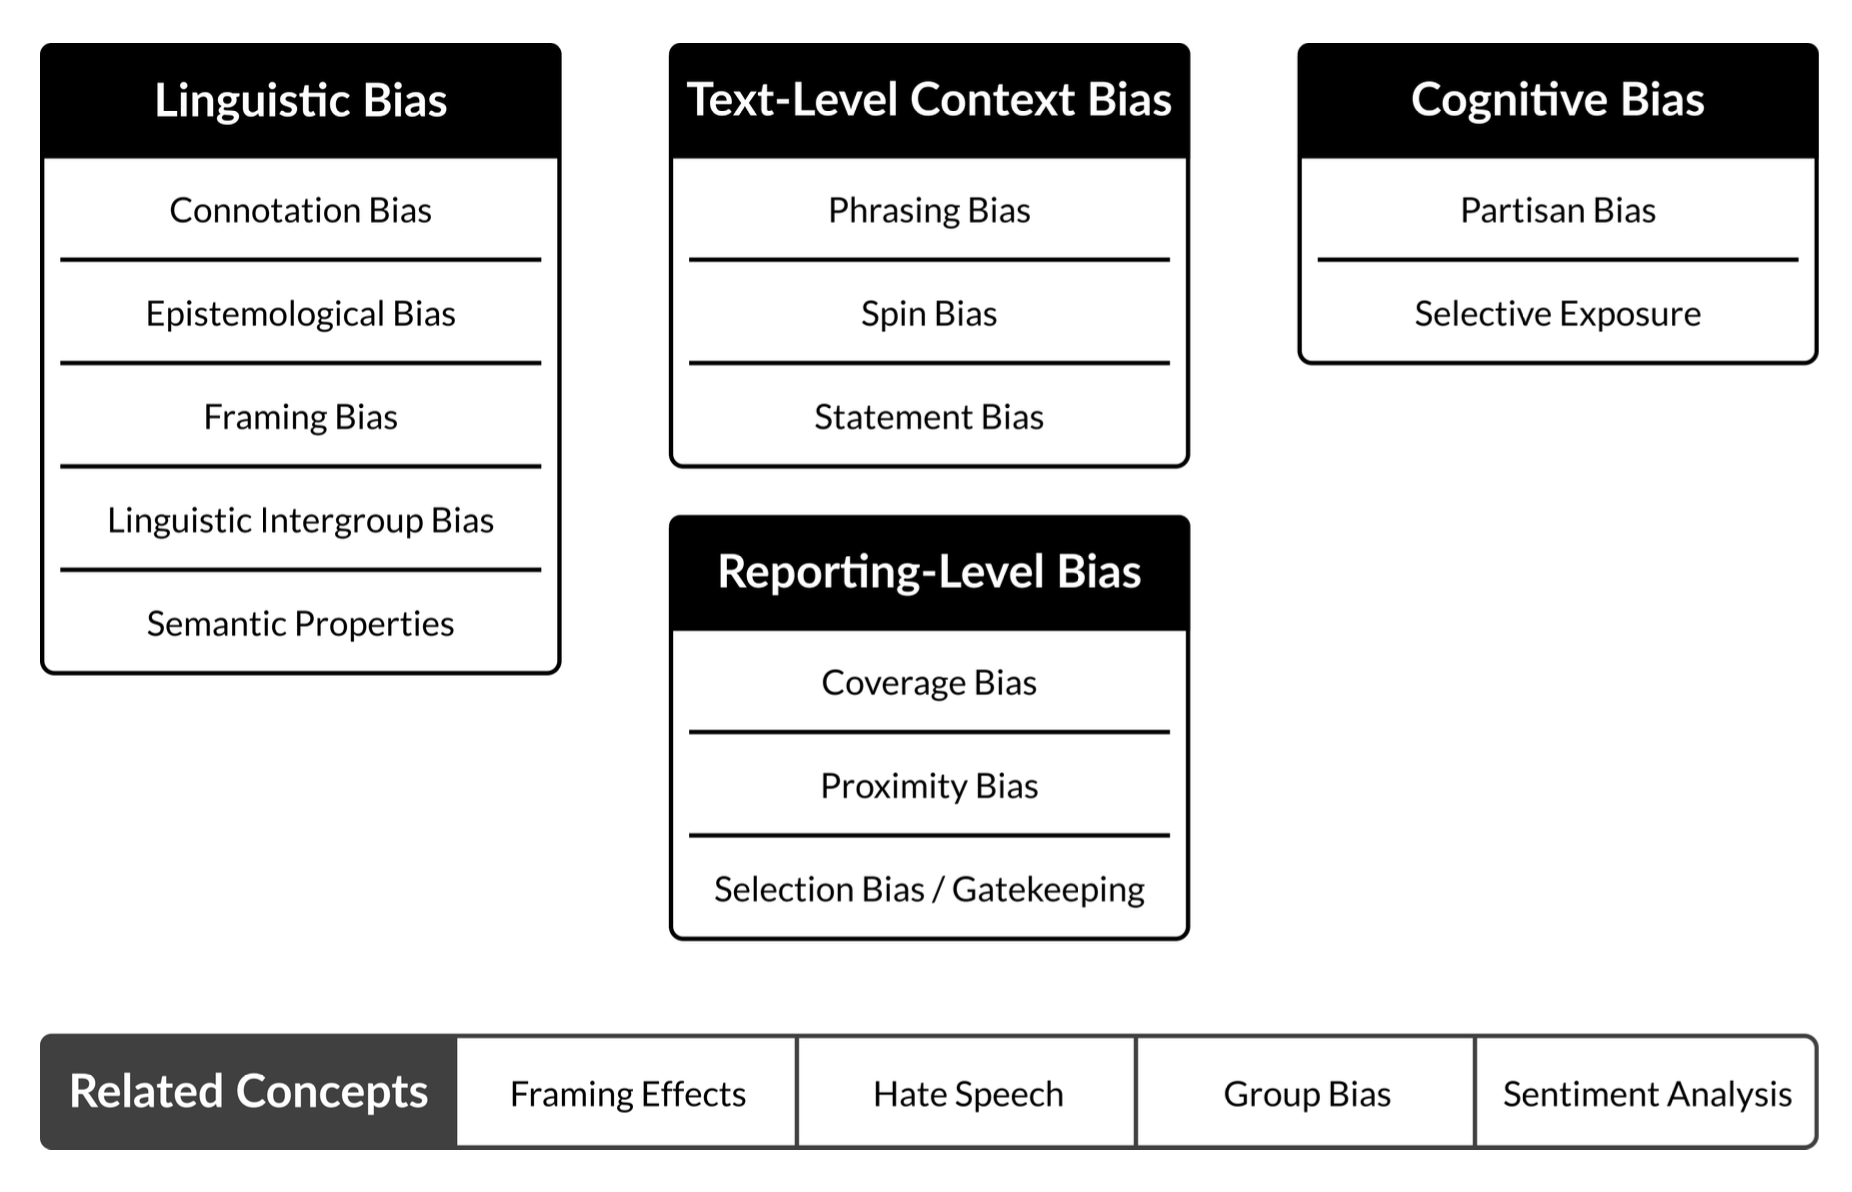
\includegraphics[width=0.9\linewidth]{images/bias-types-taxonomy.png}
    \caption{Media bias types as defined in \cite{spinde-2024-taxonomy}}
    \label{fig:bias-types-taxonomy}
\end{figure}


An example of a biased article can be seen from a recent article published by The Economist in Figure \ref{fig:the-economist-biased-article}. The headline includes a negative framing of certain groups, which can influence readers' perceptions before they even read the article, suggesting that the existence of these groups is inherently problematic and harmful. Terms like "incels" (involuntary celibates) and "anti-feminists" carry strong negative connotations, which can evoke emotional responses and suggest a negative view of the groups mentioned. This is a strong example of framing bias.

\begin{figure}[htbp]
    \centering
    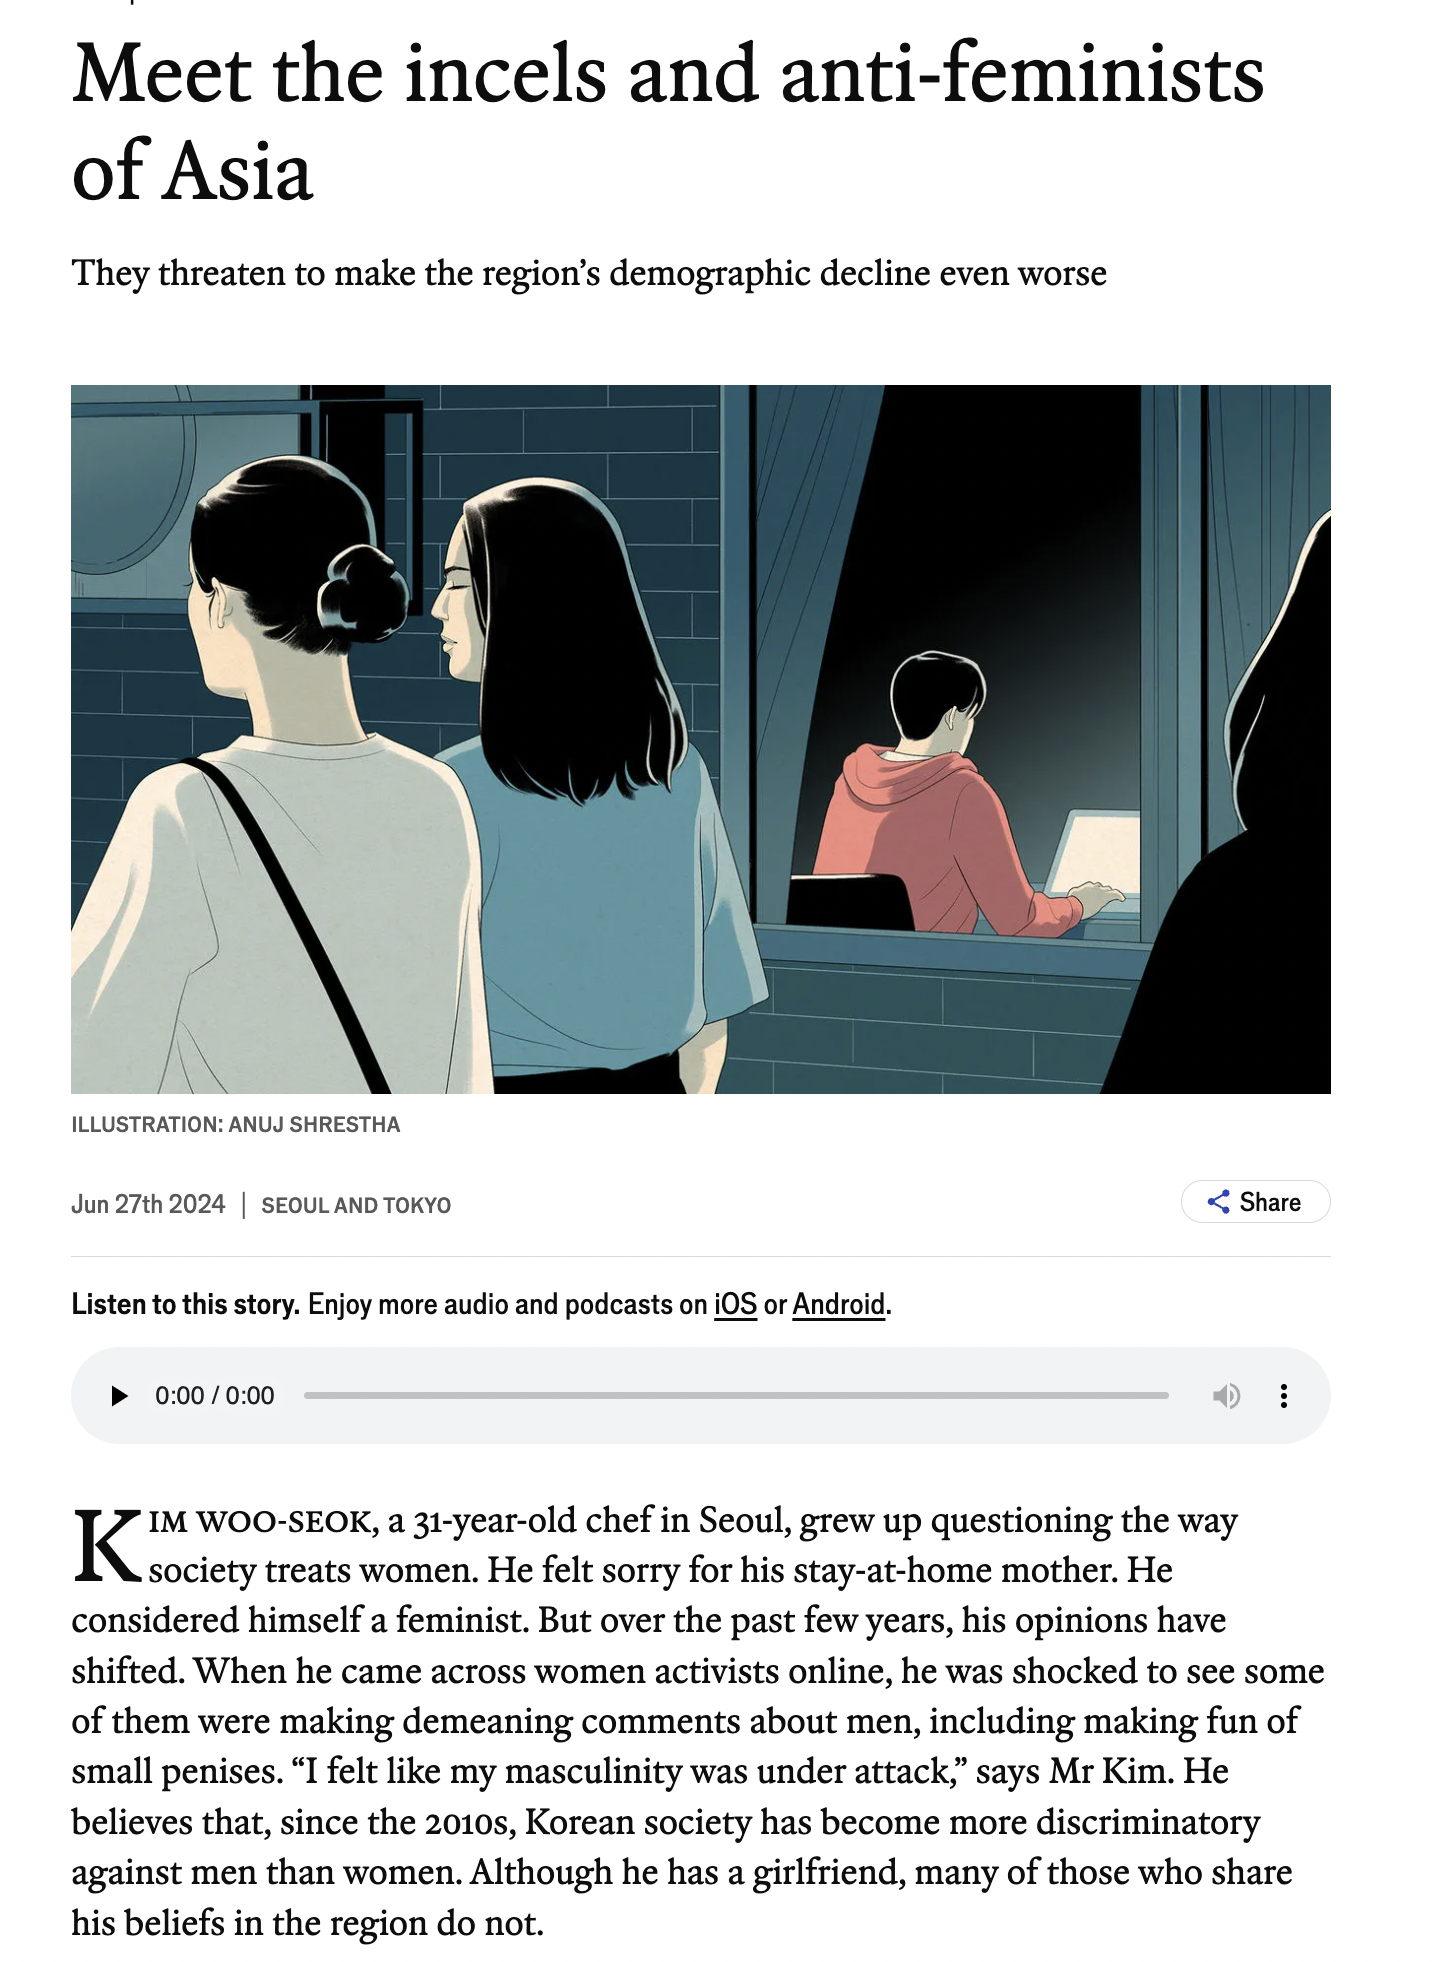
\includegraphics[width=0.9\linewidth]{images/the-economist-biased-article.png}
    \caption{A recent article from The Economist portraying gender discrimination with negative-framing headline}
    \label{fig:the-economist-biased-article}
\end{figure}

This project will mainly focus to address text-level context bias: phrasing bias, spin bias, and statement bias \cite{spinde-2024-taxonomy}: statement bias refers to “members of the media interjecting their own opinions into the text”, phrasing bias is characterised by inflammatory words, i.e., non-neutral language, spin bias describes a form of bias introduced either by leaving out the necessary information.

\section{Application}

Another particularly dangerous example of media bias is its application in relation to elections. According to a survey done by \cite{allcott-2017-socialmedia-2016election}, fake news propagated in social media played a pivotal role in the eventual election of President Trump during the 2016 election. Panagopoulos' study \cite{panagopoulos-2020} revealed systemic biases leaning towards Democratic candidates during national and state levels pre-election polls conducted during the 2020 U.S. general election cycle. Rafail et al. \cite{rafail-2018-tea-party} examined 201,678 media documents from Tea Party organizations, Fox News, MSNBC, and 785 newspapers, revealing significant differences in how the Tea Party frames itself compared to how other media sources frame the movement, MSNBC portrays it as the worst aspect of the Republican Party, while Fox News sees it as the best, sharply in contrasts with how activists frame the movement as conservative but not strictly Republican, often clashing with Republican Party goals. An analysis by Pew Research Center \cite{pew-2021-election2020} found that miscalculations observed in the 2020 U.S. election polls would adjust public opinion on issues by an average of just under 1 percentage point. Although errors of such scale would not have produced substantial differences on the American public opinions, this shows the underlying bias within polls specifically and the failure of accurately representing surveys.

The phenomenon of media bias in media has not gone unnoticed, particularly by readers and consumers, lowering public trust in media outlets. In the United States particularly, trust in news media is at an all time low, falling consistently and significantly over the past 20 years \cite{pew-2021-partisan-divides, gallup-knight-2020-american-views, reuters-2023-digital-news-report}. Approximately half of Americans believe that the media is significantly responsible for the political divisions within the United States, with a growing number of Americans losing faith in the media's objectivity and perceiving it as actively engaging in ideological wars \cite{gallup-knight-2020-american-views}. Reuters Institute reported only less than half of their respondents (40\%) generally trust the majority of news sources, with the US ranked on 29 out of 40 countries (32\%) \cite{reuters-2023-digital-news-report,reuters-2023-trust}, ranking far below developing countries such as Indonesia, Phillipines, and Turkey (full figure shown in Figure \ref{fig:trustworthiness-of-news-media-worldwide-2023}).


Readers themselves are not exempt from bias, as they are known to prefer to pick, follow, and consume articles that align with their own beliefs and ideology, an issue known as filter bubble \cite{lim-2018-understanding} or selective exposure \cite{spinde-2024-taxonomy}. This can be dangerous as it reinforces existing biases and limits exposure to diverse perspectives, creating echo chambers that hinder critical thinking and informed decision-making. The combination of media bias and filter bubbles can distort reality, perpetuate misinformation, and deepen societal divisions. It is essential for readers to seek out a variety of sources and viewpoints to gain a more balanced and comprehensive understanding of the issues at hand.


\begin{figure}[htbp]
    \centering
    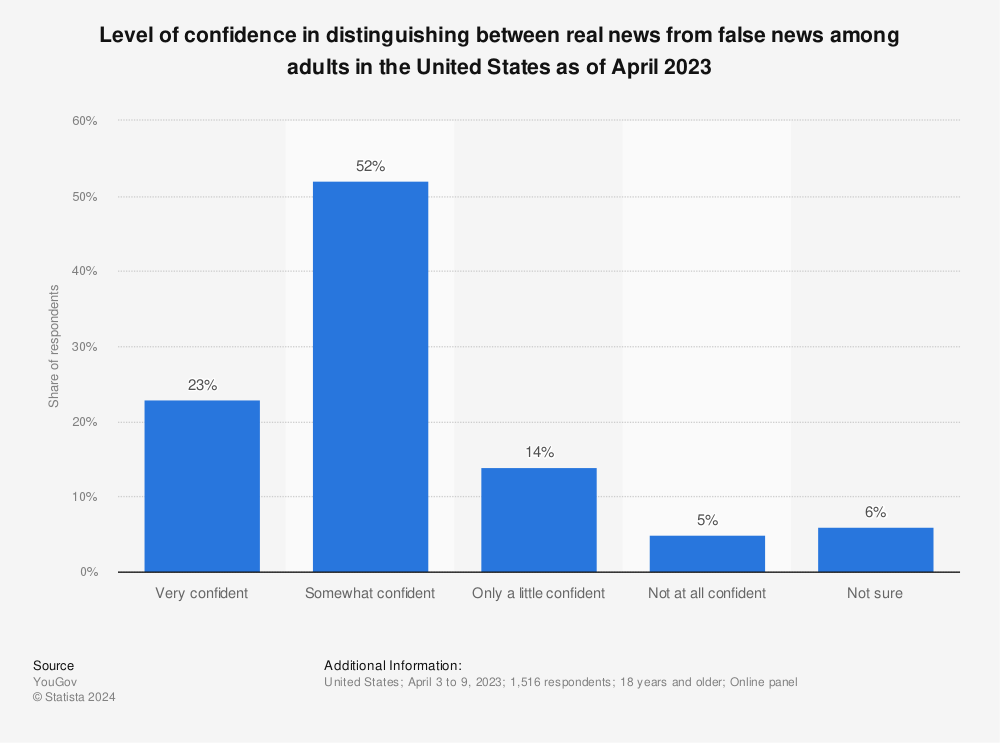
\includegraphics[width=0.9\linewidth]{images/statistic_id657090_ability-to-recognize-false-information-and-news-in-the-us-2023.png}
    \caption{Ability to recognise false information in the US \cite{yougov-2023-confidence}}
    \label{fig:ability-to-recognize-false-information-and-news-in-the-us-2023}
\end{figure}


\begin{figure}[htbp]
    \centering
    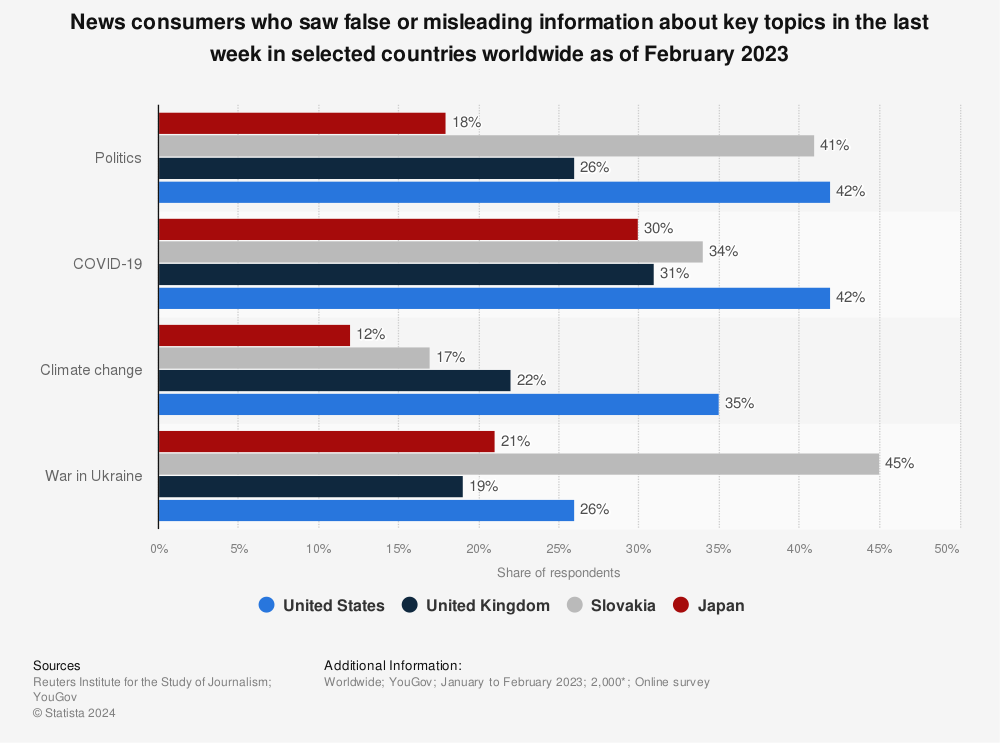
\includegraphics[width=0.9\linewidth]{images/statistic_id1317019_consumers-witnessing-false-information-on-certain-topics-worldwide-2023.png}
    \caption{\cite{reuters-2023-false-info}}
    \label{fig:consumers-witnessing-false-information-on-certain-topics-worldwide-2023}
\end{figure}


\begin{figure}[htbp]
    \centering
    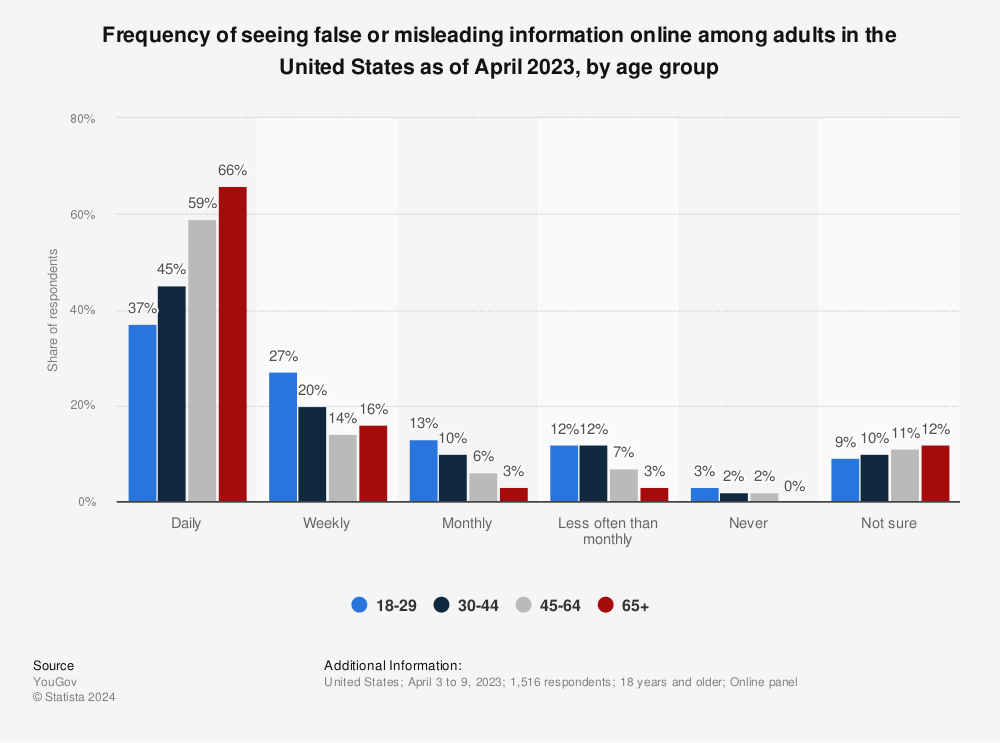
\includegraphics[width=0.9\linewidth]{images/statistic_id1462057_frequency-of-seeing-false-information-online-in-the-us-2023-by-age-group.png}
    \caption{\cite{yougov-2023-frequency}}
    \label{fig:frequency-of-seeing-false-information-online-in-the-us-2023-by-age-group}
\end{figure}

\section{Goal}

Ideally, unbiased media content that objectively and fairly represents multiple or a range of perspectives is desirable, news sources should remain neutral and let readers build their own opinions on the subject \cite{reuters-2021-digital-news-report}. However, this is often unachievable due to human capabilities and resource limitations; journalists cannot possibly possess complete knowledge on every topic, be physically present everywhere, or interview every relevant individual on a significant subject. \cite{allsides-2022-bias-definition}. Truth and journalism objectivity is a complex matter full of choices and dilemmas, where ultimately it falls on the journalists' own preferences and criteria \cite{boudana-2011-journalistic-objectivity}.

Therefore, instead of eliminating media bias, our goal should be to draw attention to its existence, giving readers awareness of such content \cite{spinde-2024-taxonomy}, ultimately building a tool to defend readers from media manipulation, to let readers know the quality of the article, and if they fall under a victim of political agenda or indoctrination.

Therefore, the primary objective of a media bias classifier should be to develop an automated system capable of classifying media bias at the article level. This system should be able to recognise and categorise bias in news articles from diverse sources, ensuring that readers are aware of what they are reading and therefore can make informed choices and opinions. The classification should encompass various dimensions of bias, including political orientation (e.g., left, right, center), sensationalism, and framing techniques.

%%% Local Variables: 
%%% mode: latex
%%% TeX-master: "thesis"
%%% End: 